\documentclass[oneside, final]{article}

\usepackage[utf8]{inputenc}
\usepackage[ukrainian]{babel}
\usepackage{hyperref}
\usepackage{url}
\usepackage{graphicx}
\usepackage{vmargin}
\setpapersize{A4}
\setmarginsrb{2cm}{1.5cm}{1cm}{1.5cm}{0pt}{0mm}{0pt}{13mm}

%opening
\title{\bf Залізничний семафор}
\author{Задворний Олексій Костянтинович}

\begin{document}

\maketitle

\begin{abstract}
\noindent Відомо, що для регулювання руху транспорту через залізничний переїзд передбачено кілька видів світлофорів.
Один з них — два мигаючих по черзі червоних сигнали.\\
Ваша задача — побудувати працюючу модель такого світлофора.\\

\noindent Проєкт призначений для молодших школярів з використанням Arduino UNO та середовища програмування mBlock або PictoBlox.
\end{abstract}

\section{Що знадобиться}
	\begin{itemize}
		\item Arduino Uno
		\item Макетна плата
		\item 2 червоних свтлодіоди
		\item 2 резистори опором 220-330 Ом
		\item З’єднувальні провода
		\item USB - кабель
	\end{itemize}

\section{Реалізація}
	\begin{enumerate}
		\item Підключить світлодіоди до макетної плати та до плати Arduino згідно схеми:
			\begin{figure}[!h]
				\centering
				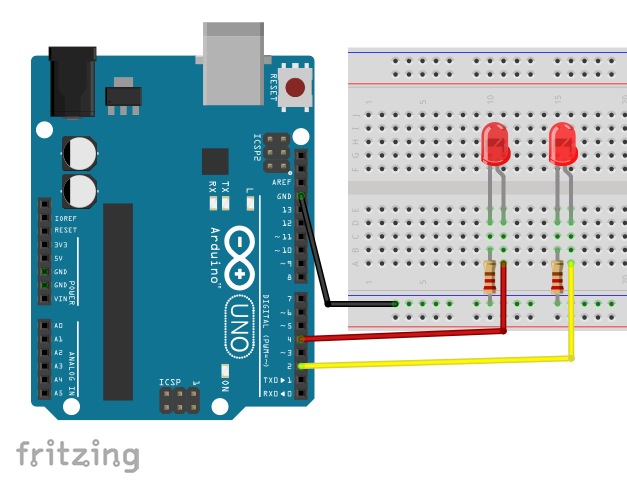
\includegraphics[scale=0.5]{circuit.png}
				\caption{Схема}
			\end{figure}
		\item Запрограмувати роботу семафора за допомогою програм mBlock або PictoBlox за схемою:
		\begin{table}
			\begin{tabular}{|c|c|}
			
			\end{tabular}
		\end{table}
	\end{enumerate}
	
\section{Поради}
	\begin{itemize}
		\item Почніть програму з блоку
			\begin{figure}[!h]
				\centering
				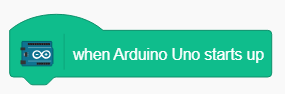
\includegraphics[scale=0.75]{UNO_start.png}
				\caption{Стартовий блок}
			\end{figure}
		\item Основні дії програми мають відбуватися у нескінченному циклі (цикл ЗАВЖДИ);
		\item Щоб увімкнути світлодіод слід подати на відповідний цифровий пін (pin) високій рівень напруги (5 В, HIGH):
			\begin{figure}[!h]
				\centering
				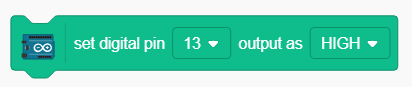
\includegraphics[scale=0.75]{setPin13HIGH.png}
				\caption{Встановлюємо HIGH на пін 13 }
			\end{figure}
		\item Щоб вимкнути світлодіод слід подати на відповідний цифровий пін (pin) низький рівень напруги (<1.5 В, LOW):
			\begin{figure}[h!]
				\centering
				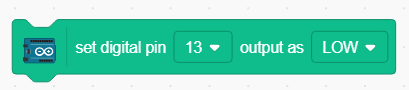
\includegraphics[scale=0.75]{setPin13LOW.png}
				\caption{Встановлюємо LOW на пін 13}
			\end{figure}
	\end{itemize}

\section{Прошивка та збереження}
	\begin{itemize}
	\item Завантажте прошивку у плату за допомогою кнопки
		\begin{figure}[h!]
			\centering
			
\includegraphics[]{upload.png}
		\end{figure}
		\\У разі виникнення проблем перевірте правильність схеми та програми.
	\item Збережіть налагоджену програму у власну папку під назвою 
\end{itemize}

\section{Посилання}
\begin{itemize}
	\item mBlock 
	\item PictoBlox 
\end{itemize}

\end{document}
